\documentclass[11pt,a4paper]{article}
\usepackage[spanish,es-tabla,es-nodecimaldot]{babel}
\usepackage[utf8]{inputenc}
\usepackage[T1]{fontenc}
\usepackage{lmodern}
\usepackage[margin=2.3cm,headheight=14pt]{geometry}
\usepackage{xcolor,graphicx,booktabs,tabularx,array,fancyhdr,titlesec,caption,enumitem}
\usepackage[most]{tcolorbox}
\usepackage[hidelinks]{hyperref}
\usepackage{microtype}

% Conmutador del borrador: \borradortrue mete las cifras de ensayo y el aviso.
\newif\ifborrador
\borradorfalse

\definecolor{verde}{HTML}{0B5A3C}
\definecolor{aviso}{HTML}{A33B00}
\definecolor{dorado}{HTML}{C8963E}
\definecolor{pendiente}{HTML}{C8963E}
\newcommand{\pend}[1]{\textcolor{pendiente}{\textbf{[#1]}}}

\titleformat{\section}{\large\bfseries\color{verde}}{\thesection.}{0.6em}{}[{\color{verde}\titlerule}]
\titleformat{\subsection}{\normalsize\bfseries\color{verde}}{\thesubsection}{0.6em}{}
\titlespacing*{\section}{0pt}{1.1em}{0.6em}
\titlespacing*{\subsection}{0pt}{0.8em}{0.3em}
\captionsetup{font=small,labelfont=bf,skip=4pt}
\setlist{nosep,leftmargin=1.4em}
\setlength{\parskip}{0.25em}

\pagestyle{fancy}
\fancyhf{}
\fancyhead[L]{\small\color{gray}Machine Learning II $\cdot$ Segunda entrega}
\fancyhead[R]{\small\color{gray}Universidad Externado de Colombia}
\fancyfoot[C]{\small\thepage}
\renewcommand{\headrulewidth}{0.4pt}

\begin{document}

% --------------------------------- portada
\begin{titlepage}
\centering
\vspace*{1.5cm}
{\color{verde}\rule{\linewidth}{1.5pt}}\\[0.5em]
{\scshape\color{verde}Universidad Externado de Colombia}\\[0.2em]
{\small\color{gray}Departamento de Matemáticas\\Ciencia de Datos}\\[0.3em]
{\color{verde}\rule{\linewidth}{0.5pt}}
\vspace{3cm}

{\large\bfseries\color{verde}Proyecto Integrador de Machine Learning II}\\[1.2em]
{\LARGE\bfseries Análisis de sentimiento en reseñas de\\[0.2em] banca digital colombiana}\\[1em]
{\itshape Reproducción y adaptación crítica de un protocolo comparativo\\ de clasificación supervisada de texto}\\[1.5em]
{\color{dorado}\rule{0.45\linewidth}{1pt}}\\[1.5em]
{\bfseries SEGUNDA ENTREGA}\\[0.3em]
Fase 2: datos, modelamiento y validación
\vfill
{\bfseries\color{verde}Integrantes}\\[0.5em]
Miguel Ángel Melo\\[0.3em]
Nicolás Mateo Corzo\\[1.5em]
\textbf{Asignatura:} Machine Learning II\\[1cm]
{\color{verde}\rule{\linewidth}{1.5pt}}
\end{titlepage}

% --------------------------------- resumen
\ifborrador
\begin{tcolorbox}[colback=aviso!8,colframe=aviso,title=\textbf{BORRADOR, no entregar},fonttitle=\small,fontupper=\small]
Las cifras de acuerdo entre anotadores de la sección 1.2 (kappa de Cohen) provienen de
\textbf{respuestas simuladas} por \texttt{src/simular\_anotacion.py}, no de una anotación real.
Sirven para ensayar el flujo y ver cómo queda el documento. Al llenar las hojas de verdad, basta
poner \texttt{\textbackslash borradorfalse} para que este aviso y esas cifras desaparezcan.
\end{tcolorbox}
\fi

\begin{tcolorbox}[colback=verde!6,colframe=verde,title=\textbf{Resumen de la entrega},fonttitle=\small,fontupper=\small]
Consolidamos un corpus real de 19\,747 reseñas de Nequi, DaviPlata y Nu (Google Play Colombia) y
un conjunto de modelado de 18\,495, con 1\,381 reseñas de una muestra anotada (oro) y 17\,114 con
etiqueta débil por estrellas, cuyo error medimos en 16,8\,\%. Al reproducir el protocolo de Alawaji y
Aloraini obtuvimos su misma exactitud (0,88 frente a 0,90), pero un F1 macro de apenas 0,45 a 0,61
sobre el oro, con modelos que nunca detectan el conflicto. Con un flujo sin fuga y validación cruzada
anidada, el mejor modelo, una regresión logística sobre n-gramas de caracteres con ponderación de
clases, alcanza un F1 macro de 0,724 $\pm$ 0,035, frente a 0,475 de la línea base, y recupera el
65\,\% de los conflictos. \ifborrador Las etiquetas de la muestra son preetiquetas asistidas por IA
revisadas por el equipo, con un kappa de Cohen de 0,63 entre los dos anotadores.\else En esta
entrega las etiquetas de la muestra son preetiquetas asistidas por IA; la revisión humana y el
kappa están en curso.\fi
\end{tcolorbox}

% ================================================================== 1
\section{Consolidación de los datos}

\subsection{Extracción y depuración}
Seguimos el procedimiento del artículo base \cite{alawaji}: con \texttt{google-play-scraper}
extrajimos el 2 de octubre de 2026 las 10\,000 reseñas más recientes de tres aplicaciones con
operación en Colombia (Nequi, DaviPlata y Nu), con tienda colombiana e idioma español. Tomamos
las más recientes, y no una muestra por estrellas, para conservar la distribución natural de las
calificaciones. La depuración (Tabla~\ref{tab:embudo}) aplica solo reglas fijas que no dependen
de la variable objetivo: anonimizamos correos, teléfonos, cédulas y nombres propios; descartamos
reseñas de menos de tres palabras, que en su mayoría son duplicados de ``excelente'' y no
contienen información para distinguir el conflicto; eliminamos duplicados exactos del texto
normalizado, para que un mismo texto no quede a la vez en entrenamiento y prueba; y filtramos
otros idiomas. Durante la anotación encontramos que la aplicación de Nu es global y que el filtro
de país deja pasar reseñas de México (mencionan el INE, la CURP o las Sofipos), por lo que
retiramos las de Nu con esos marcadores.

\begin{table}[h]
\centering\small
\caption{Embudo de depuración del corpus.}\label{tab:embudo}
\begin{tabular}{lrr}
\toprule
Paso & Reseñas & Retiradas \\
\midrule
Extraídas (3 aplicaciones $\times$ 10\,000) & 30\,000 & \\
Con texto & 29\,999 & 1 \\
Tres palabras o más & 21\,369 & 8\,630 \\
Sin duplicados exactos & 19\,897 & 1\,472 \\
En español & 19\,891 & 6 \\
Sin reseñas de México (Nu) & \textbf{19\,747} & 144 \\
\bottomrule
\end{tabular}
\end{table}

\subsection{Etiquetado y verificación de la etiqueta débil}
La Entrega 1 planteaba una etiqueta débil por estrellas (una y dos, negativa; cuatro y cinco,
positiva) y anotación manual de las reseñas de tres estrellas como candidatas a conflicto. Para
verificar ese supuesto etiquetamos una muestra de 1\,440 reseñas: todas las de tres estrellas
y 75 aleatorias de cada uno de los otros niveles. Las hojas de anotación no muestran las estrellas,
para no sesgar al anotador. La muestra se preetiquetó con asistencia de IA siguiendo una guía escrita
con definiciones y reglas para casos dudosos (por ejemplo, ``funcionaba bien, desde la
actualización no abre'' es conflicto; ``antes ingresaba normal'' no lo es). Los resultados de esta
entrega usan esas preetiquetas.
\ifborrador
Para medir su confiabilidad, cada integrante anotó por separado y a ciegas un subconjunto
estratificado de 120 reseñas, sin ver las estrellas ni la preetiqueta. El kappa de Cohen entre
nosotros fue de 0,63, con un acuerdo simple del 82\,\%, y el de cada uno frente a la preetiqueta
asistida fue de 0,84 y 0,74. Los 22 desacuerdos, concentrados casi todos en la frontera entre
negativa y conflicto, se resolvieron por consenso. El resto de la muestra se revisó fila por fila.
\else
La validación humana está en curso con dos mecanismos: cada
integrante anota por separado y a ciegas un subconjunto estratificado de 120 reseñas, del que
saldrá el kappa de Cohen entre nosotros y frente a la preetiqueta, y el resto se revisa fila por
fila. El flujo está preparado para que, al terminar la revisión, todas las cifras se recalculen
con un solo comando; los cambios se reportarán en la entrega final.
\fi

\begin{figure}[h]
\centering
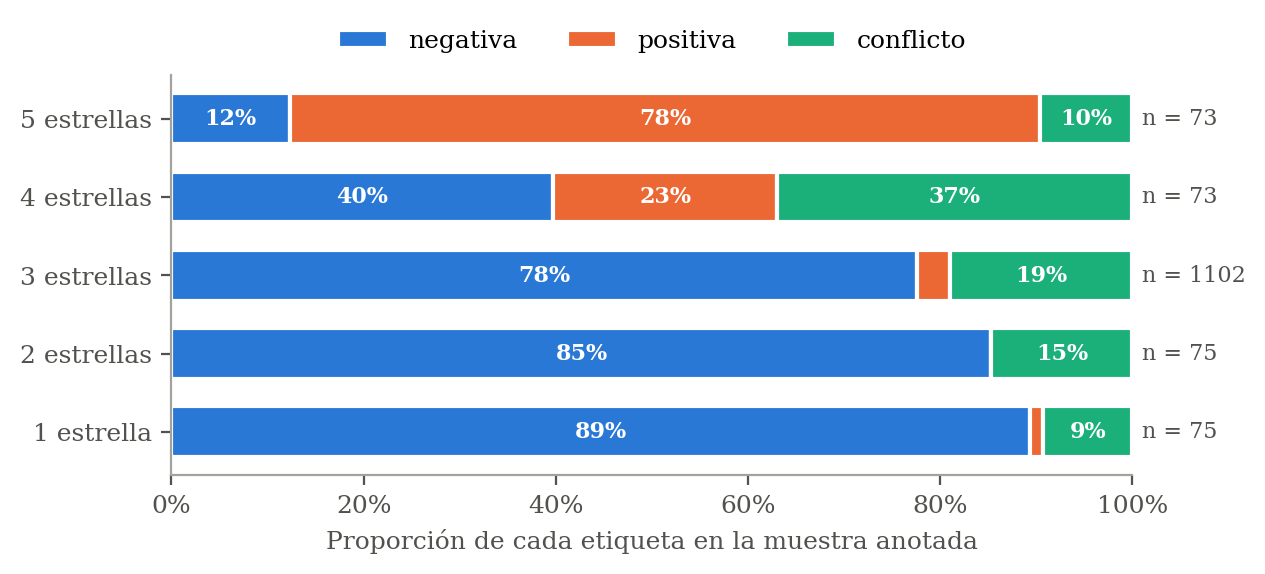
\includegraphics[width=0.82\linewidth]{../reports/figures/fig1_estrellas_vs_etiqueta.png}
\caption{Etiqueta de la muestra anotada según la calificación en estrellas (muestra anotada). Las filas de 1, 2,
4 y 5 estrellas son muestras aleatorias, por lo que estiman la exactitud de la etiqueta débil.}
\label{fig:estrellas}
\end{figure}

La verificación refutó dos supuestos de la Entrega 1 (Figura~\ref{fig:estrellas}). Primero, tres
estrellas no equivale a sentimiento mixto: el 78\,\% de esas reseñas son quejas, en buena parte por
las fallas de DaviPlata de mayo y julio de 2026 (meses con 1\,856 y 2\,695 reseñas de esa
aplicación, frente a unas 400 en un mes típico), y solo el 19\,\% son conflicto. Segundo, la regla
``cuatro estrellas, positiva'' acierta apenas en el 24\,\% de los casos: el 40\,\% de esas reseñas
son quejas y el 37\,\% son conflicto. Por eso excluimos las reseñas de cuatro estrellas que no
fueron anotadas y conservamos la etiqueta débil solo donde es razonable (1 y 2 estrellas, con
aciertos del 89\,\% y 85\,\%; 5 estrellas, con 78\,\%). Ponderando por el número de reseñas de cada
nivel, estimamos que el 16,8\,\% de las etiquetas débiles que usamos son incorrectas. Esa es la
cota de ruido del corpus, y la razón por la que toda métrica de selección y de evaluación la
calculamos solo sobre la muestra anotada (el oro).

\subsection{Conjunto definitivo y calidad}
El conjunto de modelado tiene 18\,495 reseñas (Tabla~\ref{tab:conjunto}): 1\,381 de la muestra
anotada (las 40 marcadas como irrelevantes se descartaron, como en el artículo) y 17\,114 con
etiqueta débil. El conflicto representa el 1,4\,\% del total, tres veces menos que en el corpus
saudí (4,35\,\%), y se concentra en el oro (18,6\,\%). La mediana de longitud es de 13 palabras en
la parte débil y de 19 en el oro. Hay dos rasgos de calidad que condicionan el análisis. El 11,8\,\%
de las reseñas no reporta versión de la aplicación. Y la ventana temporal difiere entre entidades:
las 10\,000 reseñas de Nequi y Nu cubren de junio y julio a octubre de 2026, mientras que las de
DaviPlata se remontan a noviembre de 2025. Además, DaviPlata aporta el 68\,\% de las negativas, lo que obliga a vigilar que el modelo
no aprenda la entidad en lugar del sentimiento. La
calificación en estrellas se conserva solo para el análisis: nunca es predictor, porque de ella
sale la etiqueta débil y usarla sería fuga directa (un error que tenía el Cuadro 6 de la
Entrega 1).

\begin{table}[h]
\centering\small
\caption{Composición del conjunto de modelado por fuente de la etiqueta y entidad.}\label{tab:conjunto}
\begin{tabular}{lrrrrrr}
\toprule
 & \multicolumn{3}{c}{Muestra anotada (oro)} & \multicolumn{2}{c}{Etiqueta débil} & \\
\cmidrule(lr){2-4}\cmidrule(lr){5-6}
Entidad & Negativa & Positiva & Conflicto & Negativa & Positiva & Total \\
\midrule
DaviPlata & 596 & 8 & 97 & 6\,126 & 1\,123 & 7\,950 \\
Nequi & 234 & 43 & 94 & 1\,534 & 2\,679 & 4\,584 \\
Nu & 184 & 59 & 66 & 1\,155 & 4\,497 & 5\,961 \\
\midrule
Total & 1\,014 & 110 & 257 & 8\,815 & 8\,299 & 18\,495 \\
\bottomrule
\end{tabular}
\end{table}

% ================================================================== 2
\section{Flujo reproducible sin fuga de información}
El flujo está en el repositorio (Anexo) y se ejecuta completo con \texttt{run\_all.sh} y semilla
42. Sus etapas, en orden, son:
\begin{enumerate}
\item \textbf{Normalización determinista} (minúsculas, sin tildes pero con ñ, números y
  alargamientos reducidos, sin emojis ni puntuación). No aprende nada de los datos, así que
  aplicarla antes de partir no filtra información.
\item \textbf{Particiones estratificadas por clase y por fuente}, para que cada pliegue tenga
  reseñas de oro de las tres clases. Los duplicados ya se eliminaron antes de partir.
\item \textbf{Pipeline}: selección de la columna de texto, TF-IDF, selección de términos por
  $\chi^2$ (solo en los modelos de árboles), SMOTE (solo cuando se compara) y clasificador. El
  vocabulario, los pesos IDF, los términos elegidos por $\chi^2$ y los ejemplos sintéticos se
  ajustan con el pliegue de entrenamiento y después se aplican sin cambios al de prueba. Esta es
  la corrección de la principal fuga posible del artículo, que no declara dónde ajustó el TF-IDF.
\item \textbf{Validación cruzada anidada}: 5 pliegues externos para estimar el desempeño y 3
  internos para elegir hiperparámetros con \texttt{GridSearchCV}. El pliegue externo de prueba
  nunca participa en la selección.
\item \textbf{Puntuación solo sobre el oro}: el entrenamiento usa todas las reseñas, pero el F1
  macro que guía la búsqueda y el que reportamos se calculan únicamente con las etiquetas
  de la muestra anotada. Así evitamos premiar a un modelo por imitar el ruido de las estrellas.
\end{enumerate}

% ================================================================== 3
\section{Reproducción y adaptación del método}

\subsection{Reproducción fiel del protocolo del artículo}
Replicamos el primer experimento de Alawaji y Aloraini tal como lo describen: TF-IDF de unigramas,
eliminación de palabras vacías con NLTK, hiperparámetros por defecto, los mismos seis modelos con y
sin ponderación de clases, voto duro sobre árbol, regresión logística y Random Forest, y CV
estratificada de cinco pliegues. Solo corregimos lo que no altera el método: el TF-IDF se ajusta
dentro de cada pliegue y agregamos el clasificador de mayoría y las métricas por clase.

\begin{figure}[h]
\centering
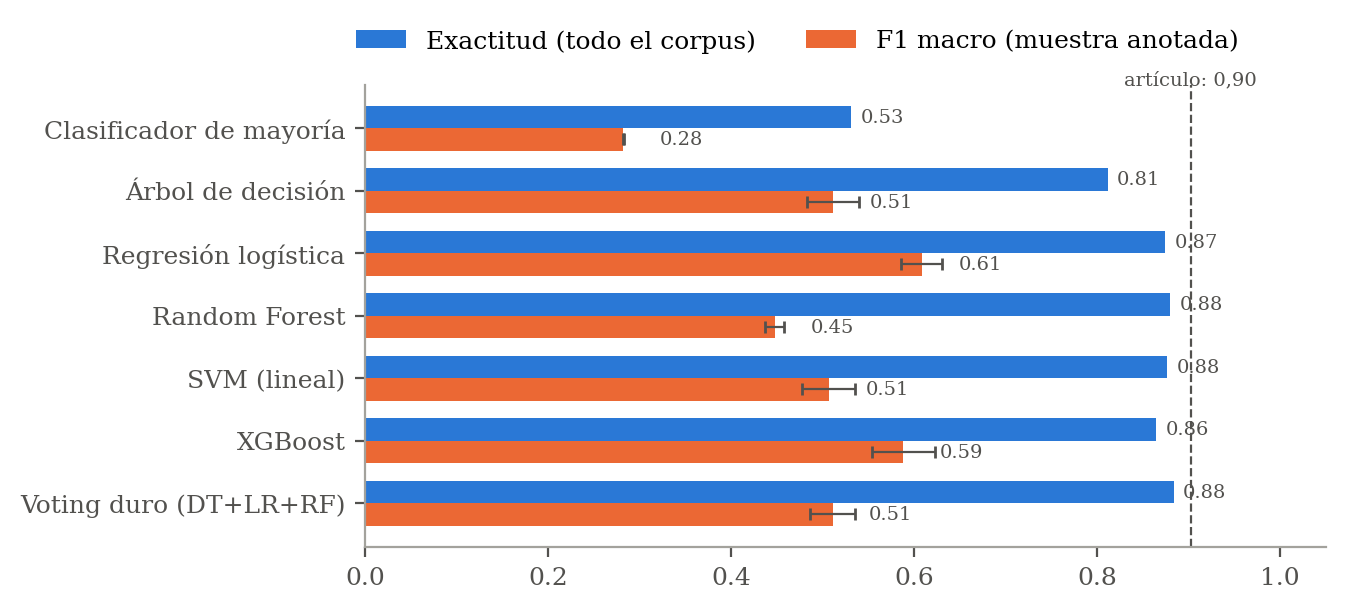
\includegraphics[width=0.84\linewidth]{../reports/figures/fig2_reproduccion.png}
\caption{Reproducción del protocolo del artículo (con ponderación de clases). La exactitud se
calcula sobre todo el corpus, como en el artículo; el F1 macro, sobre la muestra anotada. Las
barras de error son la desviación estándar entre pliegues.}
\label{fig:repro}
\end{figure}

El resultado reproduce el titular del artículo y, a la vez, su principal debilidad
(Figura~\ref{fig:repro}). La exactitud queda entre 0,81 y 0,88, muy cerca del 0,90 reportado, y la
regresión logística, la SVM y el voto quedan prácticamente empatados, como en el estudio saudí. Pero
el F1 macro sobre las reseñas de oro cae a un rango de 0,45 a 0,61, y sin ponderación la regresión
logística, el Random Forest y el voto obtienen un F1 de \emph{cero} en la clase conflicto: alcanzan
una exactitud de entre 88 y 89\,\% sin reconocer una sola reseña mixta. La ponderación es la que más ayuda
(la regresión logística pasa de 0,46 a 0,61 de F1 macro), lo que confirma el hallazgo del artículo,
salvo en el Random Forest, cuyos árboles crecen hasta hojas puras y casi no cambian con los
pesos. La conclusión es la misma que
anticipamos en la Entrega 1: la exactitud agregada del artículo no informa sobre la clase que le da
sentido al problema.

\subsection{Adaptación: representación del texto y tratamiento del desbalance}
Con dos clasificadores lineales y parámetros por defecto aislamos el efecto de la representación y
del desbalance (Figura~\ref{fig:rep}). Hay tres hallazgos. Primero, eliminar palabras vacías, como
hace el artículo, \emph{empeora} el modelo: la lista de NLTK borra ``no'', ``pero'', ``sin'' y
``nada'', que son precisamente las marcas de la negación y del contraste; conservarlas sube el F1
macro de la regresión logística de 0,61 a 0,67. Segundo, los bigramas (0,69) y los n-gramas de
caracteres (0,70) capturan la negación y son robustos a la ortografía informal (``exelente'',
``aveces''), lo que corrige la contradicción del artículo entre su exploración, que destaca
bigramas, y su modelo de unigramas. Tercero, la ponderación de clases iguala o supera a SMOTE en la
regresión logística, y es preferible porque no fabrica vectores TF-IDF que no corresponden a ningún
texto; en la SVM, en cambio, SMOTE rinde más, una señal de que su $C$ por defecto sobreajusta y
necesita ajuste. Con esto, la adaptación respeta el propósito del método (comparar familias de
clasificadores sobre TF-IDF con tratamiento del desbalance) y modifica lo que el contexto exige:
español coloquial, una clase minoritaria tres veces más escasa y etiquetas con ruido medido.

\begin{figure}[h]
\centering
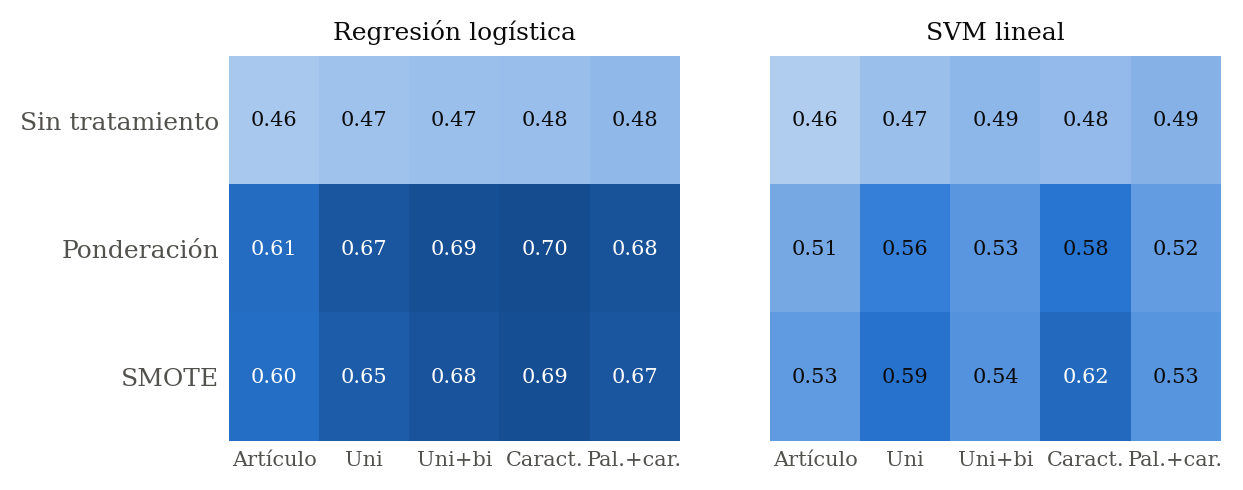
\includegraphics[width=0.86\linewidth]{../reports/figures/fig3_representacion.png}
\caption{F1 macro sobre la muestra anotada según la representación y el tratamiento del desbalance
(media de 5 pliegues). Artículo: unigramas sin palabras vacías; Uni: unigramas; Uni+bi: uni y
bigramas; Caract.: n-gramas de caracteres de 2 a 5; Pal.+car.: unión de ambos.}
\label{fig:rep}
\end{figure}

% ================================================================== 4
\section{Validación, métricas e interpretación preliminar}

\subsection{Comparación de modelos con validación cruzada anidada}
La métrica principal es el \textbf{F1 macro sobre el oro}: pondera igual las tres clases, de modo
que un modelo no puede puntuar alto ignorando el conflicto, y se calcula sobre las etiquetas en
las que confiamos. Reportamos además el F1 de la clase conflicto, porque es la de mayor costo
operativo (es la queja puntual dentro de un servicio que el usuario valora), y la exactitud
sobre todo el corpus solo como referencia frente al artículo. Todas las cifras son la media y la
desviación estándar de los 5 pliegues externos. Los modelos de árboles reciben los 3\,000 términos
con mayor $\chi^2$ del pliegue, porque los cortes univariados sobre decenas de miles de
dimensiones dispersas son lentos y ruidosos; los ensambles combinan una regresión logística sobre
caracteres, una SVM calibrada sobre palabras y LightGBM, cada uno con su propia representación.

\begin{table}[h]
\centering\small
\caption{Validación cruzada anidada (5 pliegues externos y 3 internos). F1 sobre la muestra anotada; exactitud sobre todo el corpus, solo como referencia frente al artículo.}\label{tab:anidada}
\begin{tabular}{lcccr}
\toprule
Modelo & F1 macro (oro) & F1 conflicto (oro) & Exactitud & Min. \\
\midrule
\textbf{Regresión logística} & \textbf{0{,}724 $\pm$ 0{,}035} & 0{,}686 $\pm$ 0{,}040 & 0{,}861 & 2{,}9 \\
Stacking & 0{,}718 $\pm$ 0{,}037 & 0{,}688 $\pm$ 0{,}027 & 0{,}846 & 8{,}1 \\
CatBoost & 0{,}687 $\pm$ 0{,}014 & 0{,}692 $\pm$ 0{,}032 & 0{,}847 & 5{,}4 \\
XGBoost & 0{,}654 $\pm$ 0{,}023 & 0{,}579 $\pm$ 0{,}027 & 0{,}872 & 8{,}6 \\
SVM lineal & 0{,}638 $\pm$ 0{,}032 & 0{,}436 $\pm$ 0{,}077 & 0{,}889 & 3{,}8 \\
LightGBM & 0{,}621 $\pm$ 0{,}039 & 0{,}474 $\pm$ 0{,}085 & 0{,}882 & 8{,}2 \\
Árbol de decisión & 0{,}602 $\pm$ 0{,}039 & 0{,}531 $\pm$ 0{,}064 & 0{,}810 & 1{,}4 \\
Voting suave & 0{,}575 $\pm$ 0{,}031 & 0{,}297 $\pm$ 0{,}039 & 0{,}898 & 3{,}5 \\
Random Forest & 0{,}553 $\pm$ 0{,}024 & 0{,}231 $\pm$ 0{,}053 & 0{,}879 & 6{,}2 \\
Reg. logística por defecto (línea base) & 0{,}475 $\pm$ 0{,}024 & 0{,}000 $\pm$ 0{,}000 & 0{,}900 & 0{,}2 \\
Mayoría (línea base) & 0{,}282 $\pm$ 0{,}000 & 0{,}000 $\pm$ 0{,}000 & 0{,}531 & 0{,}1 \\
\bottomrule
\end{tabular}
\end{table}

\begin{figure}[h]
\centering
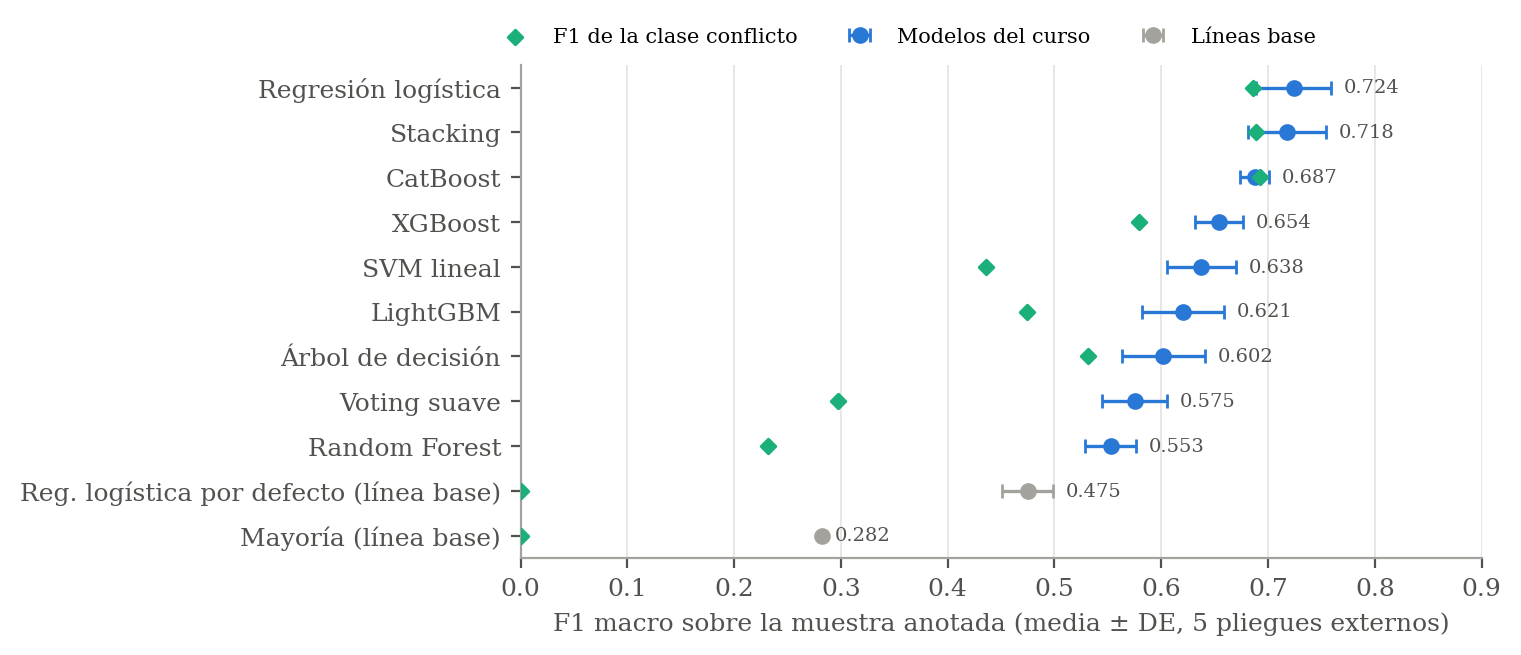
\includegraphics[width=0.84\linewidth]{../reports/figures/fig4_modelos_anidada.png}
\caption{F1 macro sobre la muestra anotada en la validación cruzada anidada (media $\pm$ desviación
estándar de los 5 pliegues externos) y F1 de la clase conflicto (rombos).}
\label{fig:anidada}
\end{figure}

La regresión logística sobre n-gramas de caracteres con ponderación de clases es el mejor modelo
(Tabla~\ref{tab:anidada} y Figura~\ref{fig:anidada}): su F1 macro es de 0,724 $\pm$ 0,035, 25
puntos por encima de la línea base de Machine Learning I (0,475) y 44 por encima del clasificador
de mayoría. Esa línea base ilustra de nuevo el problema del artículo: logra una exactitud de 0,90,
la misma que reportan Alawaji y Aloraini, con un F1 nulo en el conflicto. El stacking (0,718) queda
empatado dentro de una desviación estándar, pero tarda casi tres veces más y es menos interpretable.
Entre los árboles, el boosting supera al árbol individual y al Random Forest (0,553), y CatBoost es
el mejor y el más estable (0,687 $\pm$ 0,014), con el F1 de conflicto más alto de la
tabla (0,692). El voto suave rinde menos que sus integrantes
(0,575): al calibrar la SVM sus probabilidades vuelven al prior de clases y, al promediar, se diluye
la ponderación que favorece al conflicto. Esto matiza el hallazgo central del artículo, que eligió
el ensamble por votación: medido por exactitud, el voto vuelve a estar entre los mejores (0,90),
pero no por detectar la clase minoritaria. Seleccionamos la regresión logística por su métrica
principal, su estabilidad (el bucle interno eligió el mismo $C$ en 4 de 5 pliegues), su costo
(3 minutos de CV anidada) y porque se interpreta directamente.

\subsection{Lectura preliminar del mejor modelo}
\textbf{Variables relevantes.} Para que los términos sean legibles, inspeccionamos los coeficientes
de la misma regresión logística sobre uni y bigramas (Figura~\ref{fig:terminos}). El conflicto se
apoya casi por completo en los conectores de contraste: ``pero'' tiene el coeficiente más alto de
todo el modelo, seguido de ``aunque'', ``es buena'', ``buena pero'' y ``había'' (de ``había
funcionado bien''). Es exactamente la información que el artículo destruye al eliminar palabras
vacías. La clase negativa se define por la negación (``no'', ``no me'', ``deja'', de ``no me
deja'') y la positiva por adjetivos de elogio, incluida la variante ``exelente''. Hay una señal de
alerta: ``nu'' aparece entre los términos positivos, porque la mayoría de las reseñas de Nu son de
cinco estrellas. El modelo está aprendiendo en parte la entidad y no solo el sentimiento.

\begin{figure}[h]
\centering
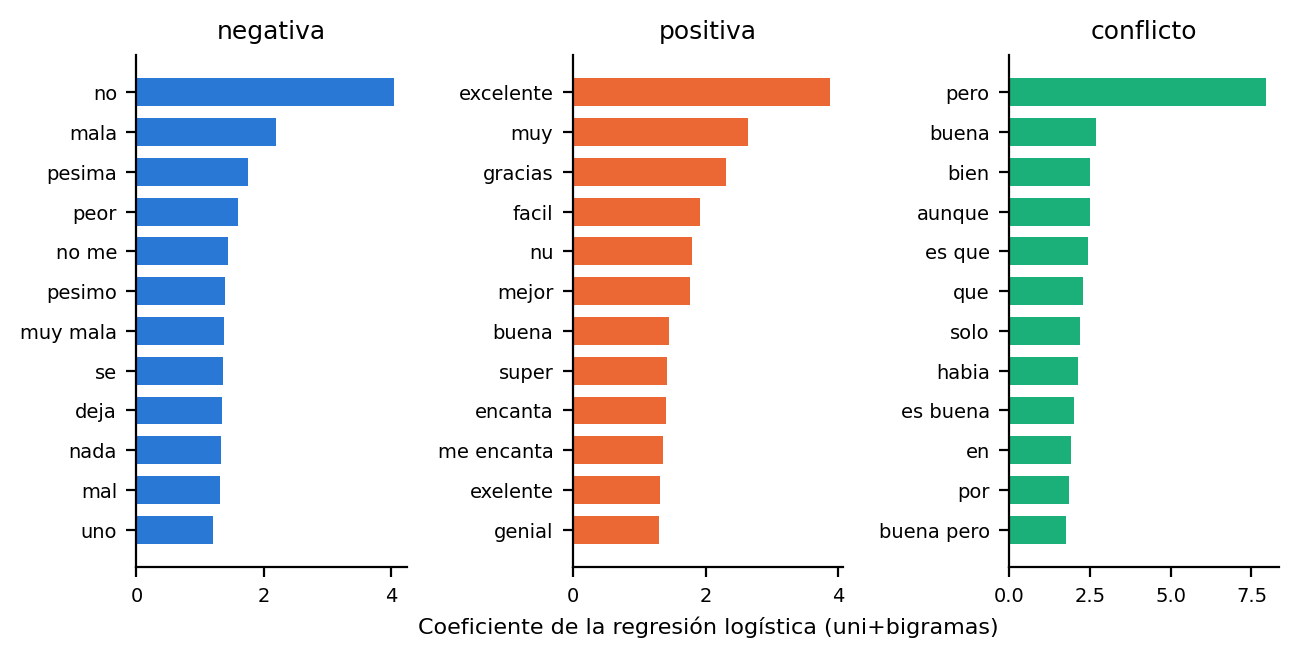
\includegraphics[width=0.86\linewidth]{../reports/figures/fig6_terminos.png}
\caption{Doce términos con mayor coeficiente por clase en la regresión logística (uni y bigramas,
$C=0{,}3$, ajustada con todo el conjunto).}
\label{fig:terminos}
\end{figure}

\textbf{Estabilidad.} El bucle interno eligió $C=0{,}3$ en 4 de los 5 pliegues, en el interior de
la rejilla, y la desviación del F1 macro entre pliegues es de 0,035. Los 25 términos principales de
cada clase se repiten entre los modelos de los cinco pliegues con un índice de Jaccard medio de 0,86
en la positiva, 0,72 en la negativa y 0,60 en el conflicto: la clase minoritaria es la menos estable,
como cabe esperar con 257 ejemplos.

\textbf{Errores.} Sumando los cinco pliegues externos (Figura~\ref{fig:confusion}), el modelo recupera
el 86\,\% de las negativas, el 91\,\% de las positivas y el 65\,\% de los conflictos, con una
precisión del 72\,\% en esta última clase. Los conflictos perdidos se reparten casi por igual entre
negativa (46) y positiva (43): son reseñas donde una de las dos partes es muy breve (``me gusta,
pero desde hace 3 días no he podido ingresar''). El error más frecuente es una negativa predicha
como positiva (88 casos), y casi siempre es una queja suave o una sugerencia con vocabulario
positivo (``si funcionará sin internet sería mejor'', ``deberian tener mas opciones y beneficios'') o una
negación que el modelo no capta (``No me gusta q ahora cobran''). Parte de estos errores
refleja una frontera discutible de nuestra guía, que clasifica las sugerencias como negativas.

\begin{figure}[h]
\centering
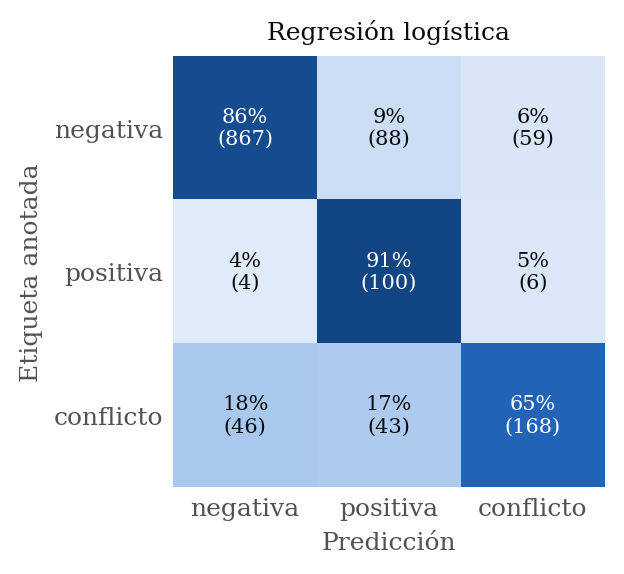
\includegraphics[width=0.42\linewidth]{../reports/figures/fig5_confusion.png}
\caption{Matriz de confusión de la regresión logística sobre la muestra anotada, sumada sobre los
5 pliegues externos (porcentaje por fila y conteo).}
\label{fig:confusion}
\end{figure}
 Por entidad, la exactitud sobre el oro es de 0,88 en DaviPlata,
0,82 en Nequi y 0,71 en Nu, coherente con la señal de entidad que detectamos en los coeficientes.

\textbf{¿Ayuda la etiqueta débil?} Con los mismos pliegues externos, la regresión logística
entrenada solo con las 1\,105 reseñas de oro de cada pliegue obtiene un F1 macro de 0,770 $\pm$
0,023, frente a 0,729 $\pm$ 0,027 con oro y etiqueta débil, y 0,738 si la parte débil pesa 0,3. Es
decir, las 13\,700 reseñas con etiqueta débil no mejoran la predicción sobre el oro. Lo atribuimos
a dos causas: su ruido (16,8\,\%) y que el oro se parece más a sí mismo que al resto del corpus,
porque sobrerrepresenta las reseñas de tres estrellas. Este resultado tiene una lectura práctica
importante: en este problema, unas pocas etiquetas confiables valen más que muchas etiquetas por
estrellas.

\subsection{Implicaciones y próximos pasos}
En términos del negocio, el modelo ya permite filtrar automáticamente las reseñas de conflicto
con algo más de una alarma falsa por cada cuatro y recuperar dos de cada tres: es útil como instrumento de
monitoreo, no como clasificador autónomo. Para la entrega final quedan cinco tareas concretas.
(1) Terminar la revisión humana de las etiquetas, calcular el kappa y recalcular todo el flujo.
(2) Evaluar el modelo final sobre un conjunto de prueba temporal: reseñas publicadas después del 2
de octubre de 2026, anotadas y nunca vistas, con la distribución natural de clases, que es el
escenario real de uso y la mejor defensa contra el sesgo temporal. (3) Enmascarar los nombres de
las entidades en el texto para que el modelo no aprenda ``nu'' como señal positiva. (4) Decidir,
con esa prueba temporal, si conviene entrenar solo con oro o mantener la etiqueta débil con menor
peso. (5) Interpretar el modelo final con SHAP y desplegarlo en Streamlit con la explicación de
cada predicción.



\section*{Anexo: código y declaración de uso de IA}
\small
Repositorio: \pend{enlace al repositorio}. Usamos Claude (Anthropic) como apoyo en la escritura de
código, el preetiquetado de la muestra (revisado por el equipo) y la revisión de redacción. Todas
las decisiones metodológicas fueron discutidas y son sustentables por ambos integrantes.

\begin{thebibliography}{9}\small
\bibitem{alawaji} Alawaji, R. y Aloraini, A. (2025). Sentiment Analysis of Digital Banking
Reviews Using Machine Learning and Large Language Models. \textit{Electronics}, 14(11), 2125.
\url{https://doi.org/10.3390/electronics14112125}
\bibitem{chawla} Chawla, N. V., Bowyer, K. W., Hall, L. O. y Kegelmeyer, W. P. (2002). SMOTE:
Synthetic Minority Over-sampling Technique. \textit{JAIR}, 16, 321-357.
\bibitem{cawley} Cawley, G. C. y Talbot, N. L. C. (2010). On Over-fitting in Model Selection and
Subsequent Selection Bias in Performance Evaluation. \textit{JMLR}, 11, 2079-2107.
\bibitem{ratner} Ratner, A. et al. (2017). Snorkel: Rapid Training Data Creation with Weak
Supervision. \textit{Proceedings of the VLDB Endowment}, 11(3), 269-282.
\bibitem{sklearn} Pedregosa, F. et al. (2011). Scikit-learn: Machine Learning in Python.
\textit{JMLR}, 12, 2825-2830.
\end{thebibliography}
\end{document}
